\documentclass{article}
\usepackage{graphicx} 
\usepackage[margin=1.0in]{geometry}
\usepackage{hyperref}

\title{
\vspace{2in}
\textmd{\textbf{AI Challenge}}\\
\normalsize\vspace{0.1in}\small{Submission due Friday, February 6}\\
\vspace{0.1in}\large{\textit{Code Camp 4.0}}
\vspace{3in}
}
\date{}


\begin{document}

\maketitle
\newpage

\section{Ants! Ants! Ants!}


Inspired by the Google AI Challenge, we present the Ant AI challenge. The idea is simple: two ant generals command an ant army, trying to capture the enemey base. Contestants will submit an agent program that commands their army. 

\section{The Board}

The board consists of five pieces

	\begin{center} 
		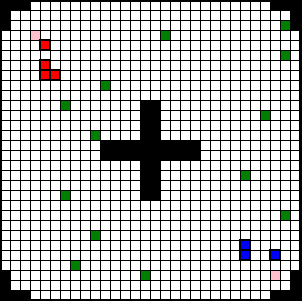
\includegraphics[scale=0.5]{exampleBoard.png}
	\end{center}

\subsection{Ants}
A player will randomly be assigned a team color: blue or red. Ants may move LEFT, RIGHT, UP or DOWN.

\subsection{Hills}
The pink squares are the hills, where new ants will spawn. Moving one of your ants on top of the opponent's hill will result in victory.

\subsection{Food}
The green squares are food, picking up a piece of food will create a new ant on your hill. If any ant is currently on your hill when you pick up a piece of food, the new ant will not spawn until the ant on top of the hill moves. Up to four new food may be spawned every turn.

\subsection{Wall}
No ants may move here, nor may food spawn here.

\subsection{Open Spaces}
Any ant may try to claim an open space. The map wraps around (i.e. an ant moving right at the rightmost boundary will appear at the leftmost boundary)

\newpage
\section{Moving}
Agents will submit a list of moves and each move will be simulated as if they happen at the same time. Moves may only take a maximum of TWO SECONDS to compute. If the agent does not send a move within the timeframe, no move is made.
\subsection{Basic Moves}
\begin{center}
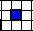
\includegraphics{basicMove.png}
\end{center}
\begin{itemize}
  \item An ant may move LEFT, RIGHT, UP or DOWN. No diagonal moves are allowed
  \item You may not move on top of a wall
  \item The map wraps around (i.e. an ant moving right at the rightmost boundary will appear at the leftmost boundary)
  \item An invalid move will result in no move
\end{itemize}


\subsection{Interacting With Other Ants}
\begin{center}
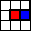
\includegraphics{fight.png}
\end{center}
\begin{itemize}
  \item Moving onto an enemy ant results in the destruction of both ants
  \item If two ants swap positions, (red moves right and blue moves left) both are destroyed
  \item Two ants on the same team may destroy each other if they move onto the same square (ants aren't very smart)
\end{itemize}

\subsection{Moving On To Food}
\begin{center}

\includegraphics{foodGrab.png}
\end{center}
\begin{itemize}
  \item Grabbing food will create a new ant on your hill
  \item If any ant is currently on your hill when you pick up a piece of food, the new ant will not spawn until the ant on top of the hill moves
  \item If two ants move on to the same piece of food, both ants are destroyed and the food is preserved. No new ant will spawn
  \item If two foods are grabbed at the same time, by the same player, the new ants will be queued up
\end{itemize}

\subsection{Capturing the Hill}
\begin{center}

\includegraphics{hillCapture.png}
\end{center}
\begin{itemize}
  \item Moving your ant on top of the enemy hill wins the game
  \item If an ant of the hill being captured occupies the hill, both ants are destroyed, but the hill lives. 
\end{itemize}


\newpage

\section{What Can My Ants See?}
Ants have pretty poor vision, so they can't see the whole board at once! Any ant can only see things up to ten squares away, including wrapping around the other side of the board. Their sense of smell also allows them to see through walls!

\begin{center}
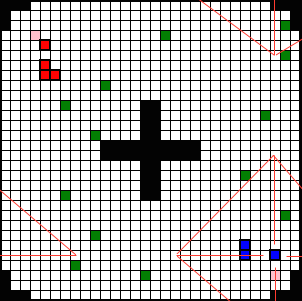
\includegraphics[scale=0.5]{fieldOfVision.png}
\end{center}

\section{Winning}
There are three ways to win a game of Ants
\begin{itemize}
  \item Destroying the opponent ant hill
  \item If both ant hills are destroyed at the same time, the player with the most ants wins
  \item If time expires on the game, the player with the most ants wins
  \item If time expires and the number of ants is equal, a tie will be declared and the game will be re-run
\end{itemize}

\section{Controlling Your Army}
\subsection{Provided Clients}
We have provided base clients for .NET, Python and Node.js. An agent may be created by inheriting AgentBase. The only public methods are Update, MoveAnt and a constructor. Web service calls and connection to the server are handled by the base class.
\newline
\newline
\href{https://github.com/eonarheim/AntAICompetition}{Link to clients}

\subsection{API}
If you are interested in writing your own client in Haskell, PL/SQL or any other language, feel free to use our well-documented \href{http://antsgame.azurewebsites.net/Help}{API}

\section{Testing Your Submission}

By way of proper API calls or inheriting from the base agents, a new, observable game will be created at \url{http://antsgame.azurewebsites.net}. Or you may clone the \href{https://github.com/eonarheim/AntAICompetition}{github repo} and run locally.
\newline
\newline
When the start() method of a test agent is called, a new game against a dummy agent will be started. 

\section{Submissions}
A valid submission will include the following
\begin{itemize}
  \item Binaries and source code for working client
  \item Binaries should run on a 64-bit Windows Machine
  \item Compilation instructions if necessary
\end{itemize}


\noindent All final submissions should be placed in //genmills/corporate/public/codecamp/antai/YOURNAME
\newline
\newline

\noindent An entry may be disqualified for the following reasons
\begin{itemize}
  \item Writing to the file system
  \item Hacking into the game server in any way
  \item  Also we reserve the right to disqualify if we determine there has been a violation of the spirit of the competition. Contact us if you are unsure.
\end{itemize}

\noindent Winners will be announced on the day of Code Camp 4.0

\section{Questions? Comments? Complaints?}

We have started a \href{https://groups.google.com/forum/#!forum/gmi-ant-ai-challenge}{Google Group} where one can discuss strategies, ask clarifying questions or any other questions related to the competition. Please direct all discussion in the \href{https://groups.google.com/forum/#!forum/gmi-ant-ai-challenge}{Google Group.}



\end{document}